\documentclass{beamer}

\mode<presentation>

{
\usetheme{Rochester}
\setbeamercovered{transparent}
}

\usecolortheme{wolverine}

\usepackage{amsmath}
\usepackage{amsfonts}
\usepackage{amssymb}
\usepackage[english]{babel}
\usepackage{graphicx}
\usepackage[utf8]{inputenc}
\usepackage[T1]{fontenc}
%\usepackage[natbib=true, style=thesis, url=false, doi=false, firstinits=true, defernumbers=true, bibstyle=numeric, title=false, sorting=ydnt, citestyle=authoryear-comp, isbn=false]{biblatex}
\usepackage{lmodern}
\usepackage{hyperref}
\usepackage{lscape}
\usepackage{multirow}
\usepackage[parfill]{parskip}
\usepackage{makeidx}
%\usepackage{times}
%\bibliography{library}
\usepackage{wrapfig}
\usepackage{pgf}
\usepackage{fancybox}
\usepackage{multimedia}
%\usepackage[]{movie15}

\newcommand{\obs}{\mathrm{obs}}
\newcommand{\pred}{\mathrm{pred}}
\newcommand{\eff}{\mathrm{eff}}
\newcommand{\intt}{\mathrm{int}}
\newcommand{\LMC}{\mathrm{LMC}}
\newcommand{\MW}{\mathrm{MW}}
\newcommand{\Cepheid}{\mathrm{Cepheid}}
\newcommand{\Anchors}{\mathrm{Anchors}}
\newcommand{\SNe}{\mathrm{SNe\,Ia}}
\newcommand{\km}{\mathrm{km}}
\newcommand{\second}{\mathrm{s}}
\newcommand{\Mpc}{\mathrm{Mpc}}
%\def\be{\begin{equation}}
%\def\ee{\end{equation}}
%\def\bea{\begin{eqnarray}}
%\def\eea{\end{eqnarray}}


\author[Martin Kunz and Valeria Pettorino (Wilmar Cardona)]{Martin Kunz and Valeria Pettorino\\ (Wilmar Cardona)}
%\institute[]{University of Geneva}
%\date{18th June, 2012}

\title[Determining $H_0$ with Bayesian hyper-parameters: preliminary results]{Determining $H_0$ with Bayesian hyper-parameters: preliminary results}
\subject{Cosmology}


\beamerdefaultoverlayspecification{<+->}

\begin{document}

\begin{frame}{\textit{Planck} (and some external data sets) constraints}
\begin{columns}
\begin{column}{0.45\textwidth}
\centering
\only<1-3>{TT+TE+EE+lowP+BAO
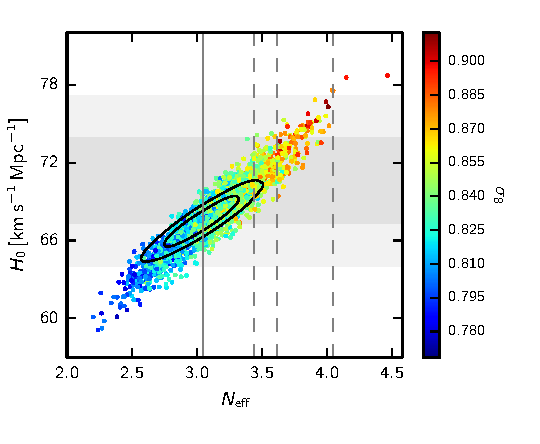
\includegraphics[scale=0.65]{./Neff-H0.pdf}
} 
\only<4-7>{TT+lowP+BAO+JLA
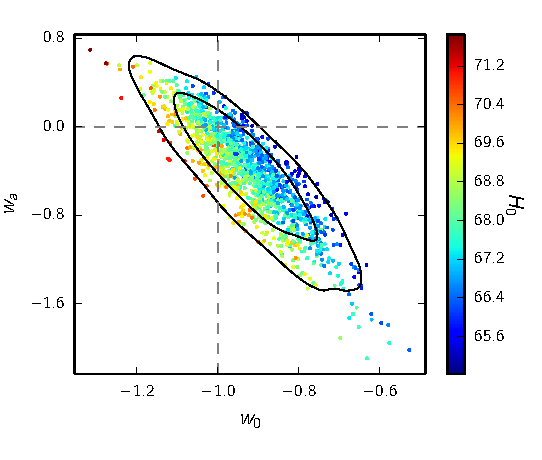
\includegraphics[scale=0.65]{./w-H0.pdf}
}
\end{column}
\begin{column}{0.45\textwidth}
\centering
\only<1-3>{TT+lowP+lensing
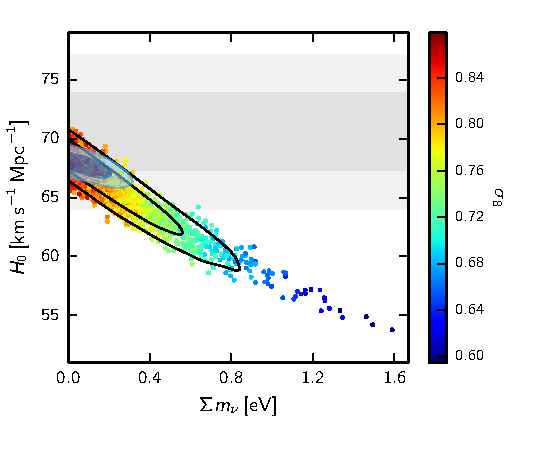
\includegraphics[scale=0.65]{./mnu-H0.pdf}} 
\only<5-7>{Direct vs. Indirect 
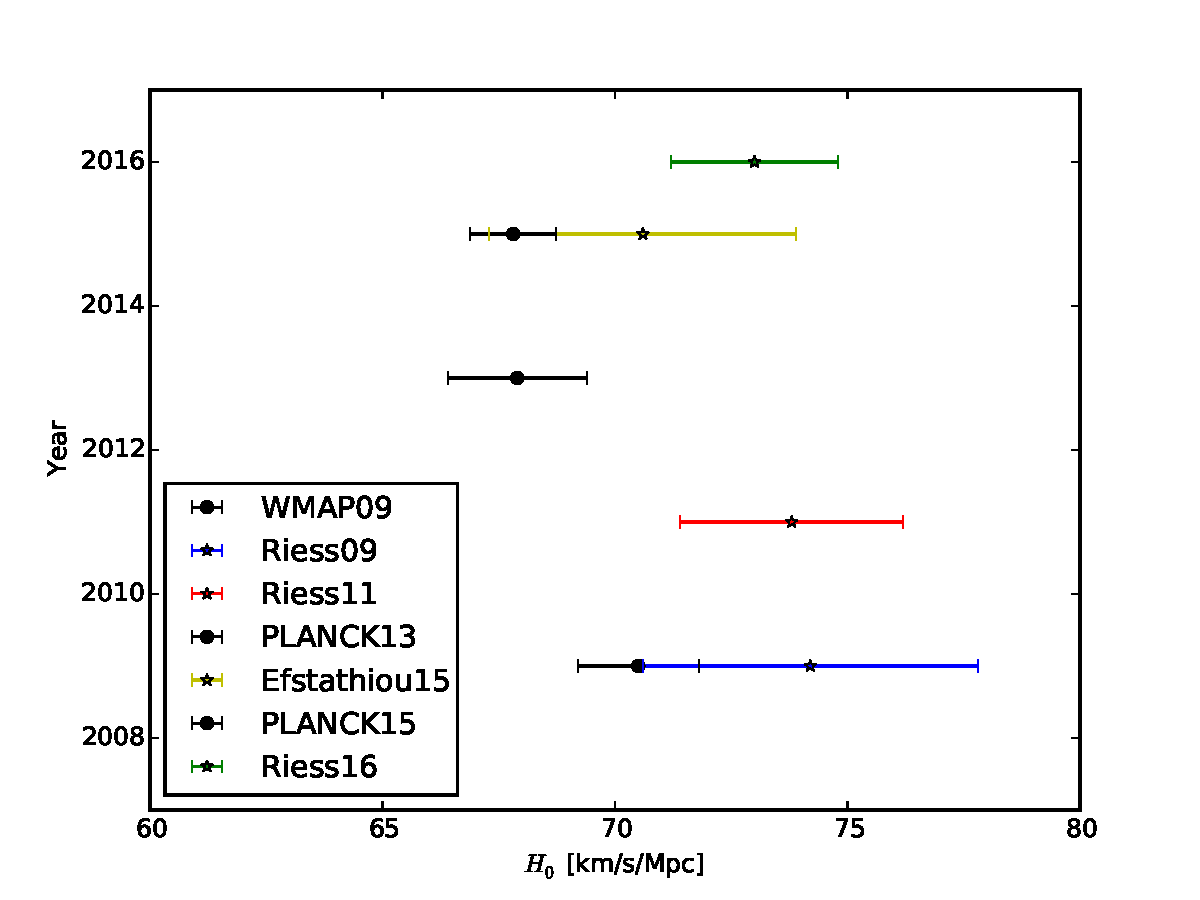
\includegraphics[scale=0.3]{./H0_values.pdf}}
%\only<4>{Inpainted NILC 
%\includegraphics[scale=0.2]{../../../../../projects/B/ksv-maps/planck-nside/nilc/192c/inpainted/vmap.pdf}}
\end{column}
\end{columns}
\begin{center}
\only<6>{Theoretical attempts ?}
\only<7>{Issues in the statistical analysis ?}
\end{center}

%A figure showing degeneracies (e.g, $w,\, m_\nu$).
%A figure comparing $H_0$ from direct measurements and from WMAP and PLANCK: WMAP9, R09, R11, PLANCK13, E15, PLANCK15. Discuss differences between R09 and R11, between R11 and E15 (rejection algorithm, new data for NGC4258), direct and derived $H_0$. Mention failed theoretical attempts to explain discrepancy by Ruth and Iggy.  
\end{frame}

\begin{frame}
  \titlepage
\end{frame}

\begin{frame}{Contents}
  \tableofcontents
\end{frame}

\section{What do you need to measure $H_0$ ?}

\begin{frame}{What do you need to measure $H_0$?}
\begin{itemize}
\item Distance modulus 
\begin{equation*}
\mu_0 = m_B - M_B = 5 \log_{10} \left(\frac{d_L}{1 \mathrm{Mpc}} \right) + 25 \, . \label{eq:distmag}
\end{equation*}
\item Cepheid variables period-luminosity relation
\begin{equation*}\label{Eq:P-L-equation}
m_{X,i,j} = \mu_{0,i} + M_X + b_X (\log P_{i,j}-1) + Z_X \Delta \log[O/H]_{i,j},
\end{equation*}
\item SN Ia magnitudes
\begin{equation*}
5 \log_{10} H_0 = m_V - \mu_0 + 5a_v + 25 \, . \label{eq:h0formalism}
\end{equation*}
\end{itemize}
\end{frame}

\section{Method: Bayesian hyper-parameters (HP)}

\begin{frame}{Method: Bayesian hyper-parameters (HP)}
\begin{itemize}
\item \textbf{Trust no one}. Some error bars may have been underestimated (e.g., unrecognised systematic effects), then allow for a rescaling $\sigma_i \rightarrow \sigma_i/\sqrt{\alpha_i}$.
\item 
\only<2>{Assume Gaussian likelihood for the data $D_i$
\begin{equation*}
P_G(D_i|\vec{w}) = \tilde{N}_i \, \frac{\exp(-\chi^2_i(\vec{w})/2)}{\sqrt{2\pi}},
\end{equation*}}
\only<3>{where  
\begin{equation*}
\chi^2_i \equiv \frac{\left( x_{\obs,i} - x_{\pred,i}(\vec{w}) \right)^2}{\sigma_i^2} \quad \mathrm{and} \quad \tilde{N}_i = \frac{1}{\sqrt{\sigma_i^2}}. 
\end{equation*}}
\only<4>{Control relative weight of data points in the likelihood with HP $\alpha_i$, likelihood becomes
\begin{equation*}
P(D_i|\vec{w},\alpha_i) = \tilde{N}_i \, \alpha_i^{1/2}\, \frac{\exp(-\alpha_i \chi^2_i(\vec{w})/2)}{\sqrt{2\pi}}.
\end{equation*}}
\only<5>{For a given model with parameters $\vec{w}$ and a set of $N$ data points $ \lbrace D_i \rbrace$ 
\begin{equation*}
P(\vec{w}|\lbrace D_i \rbrace) = \int \dots \int P(\vec{w},\lbrace \alpha_i \rbrace|\lbrace D_i \rbrace)\, d\alpha_1 \dots d\alpha_N,
\end{equation*}}
\only<6>{From Bayes' theorem
\begin{equation*}
P(\vec{w},\lbrace \alpha_i \rbrace|\lbrace D_i \rbrace) = \frac{P(\lbrace D_i \rbrace|\vec{w},\lbrace \alpha_i \rbrace)\, P(\vec{w},\lbrace \alpha_i \rbrace)}{P(D_1,\dots,D_N)},
\end{equation*}
\begin{equation*}
P(\vec{w},\lbrace \alpha_i \rbrace) = P(\vec{w}|\lbrace \alpha_i \rbrace)\, P(\lbrace \alpha_i \rbrace),
\end{equation*}
\begin{equation*}
P(\lbrace D_i \rbrace|\vec{w},\lbrace \alpha_i \rbrace)  = P(D_1|\vec{w},\alpha_1)\dots P(D_N|\vec{w},\alpha_N),
\end{equation*}
\begin{equation*}
P(\vec{w}|\lbrace \alpha_i\rbrace)  = \mathrm{constant}
\end{equation*}
\begin{equation*}
P(\lbrace \alpha_i \rbrace) = P(\alpha_1)\dots P(\alpha_N)
\end{equation*}
}
\only<7>{Further assuming uniform prior for HP ($P(\alpha_i)=1$) and that errors are never smaller than their reported value ($\alpha_i \in [0,1]$)
\begin{equation*}
P(\vec{w},\lbrace D_i \rbrace) = \frac{P(D_1|\vec{w})\dots P(D_N|\vec{w})}{P(D_1,\dots,D_N)},
\end{equation*}
\begin{equation*}
P(D_i|\vec{w}) \equiv \int_0^1 P(D_i|\vec{w},\alpha_i)\, d\alpha_i.
\end{equation*}
}
\only<8>{In the case of a Gaussian HP likelihood
\begin{equation*}
P(D_i|\vec{w}\,) = \tilde{N}_i \, \left(\frac{ \mathrm{Erf}\left( \frac{\chi_i(\vec{w})}{\sqrt{2}} \right)  -\sqrt{\frac{2}\pi} \chi_i(\vec{w}) \exp(-\chi^2_i(\vec{w})/2)}{ \chi^3_i(\vec{w})} \right)
\end{equation*}
}
\only<9>{Rewriting
\begin{equation*}
\ln P(\vec{w},\lbrace D_i \rbrace) = \sum_i \ln \tilde{N}_i + \ln \tilde{\chi}^2_i
\end{equation*}
\begin{equation*}
\tilde{\chi}^2_i(\chi^2_i(\vec{w})) \equiv \frac{ \mathrm{Erf}\left( \frac{\chi_i(\vec{w})}{\sqrt{2}} \right)  -\sqrt{\frac{2}\pi} \chi_i(\vec{w}) \exp(-\chi^2_i(\vec{w})/2)}{ \chi^3_i(\vec{w})}
\end{equation*}
}
\only<10>{Effective HP for each data point are given by
\begin{eqnarray*}
\alpha^{\eff}_i & = 1,\quad \mathrm{if} \quad \chi^2_i\leq1
\\
\label{Eq:effective-HP-2}
\alpha^{\eff}_i & = \frac{1}{\chi^2_i},\quad \mathrm{if} \quad \chi^2_i> 1.
\end{eqnarray*}
}
\end{itemize}

\end{frame}

\section{Applying HP: Period-Luminosity relation}

%\begin{frame}{Applying HP: Cepheid variables}{P-L relation}
%Period luminosity relation, distance modulus, apparent magnitude for SN Ia
%\includegraphics[scale=0.4]{../../../../../projects/B/cmb-maps/planck-nside/gaussian/map_2000.pdf} 
%\end{frame}

\begin{frame}{Applying HP}{Large Magellanic Cloud (LMC)}
 
 
\only<1>{LMC figure}%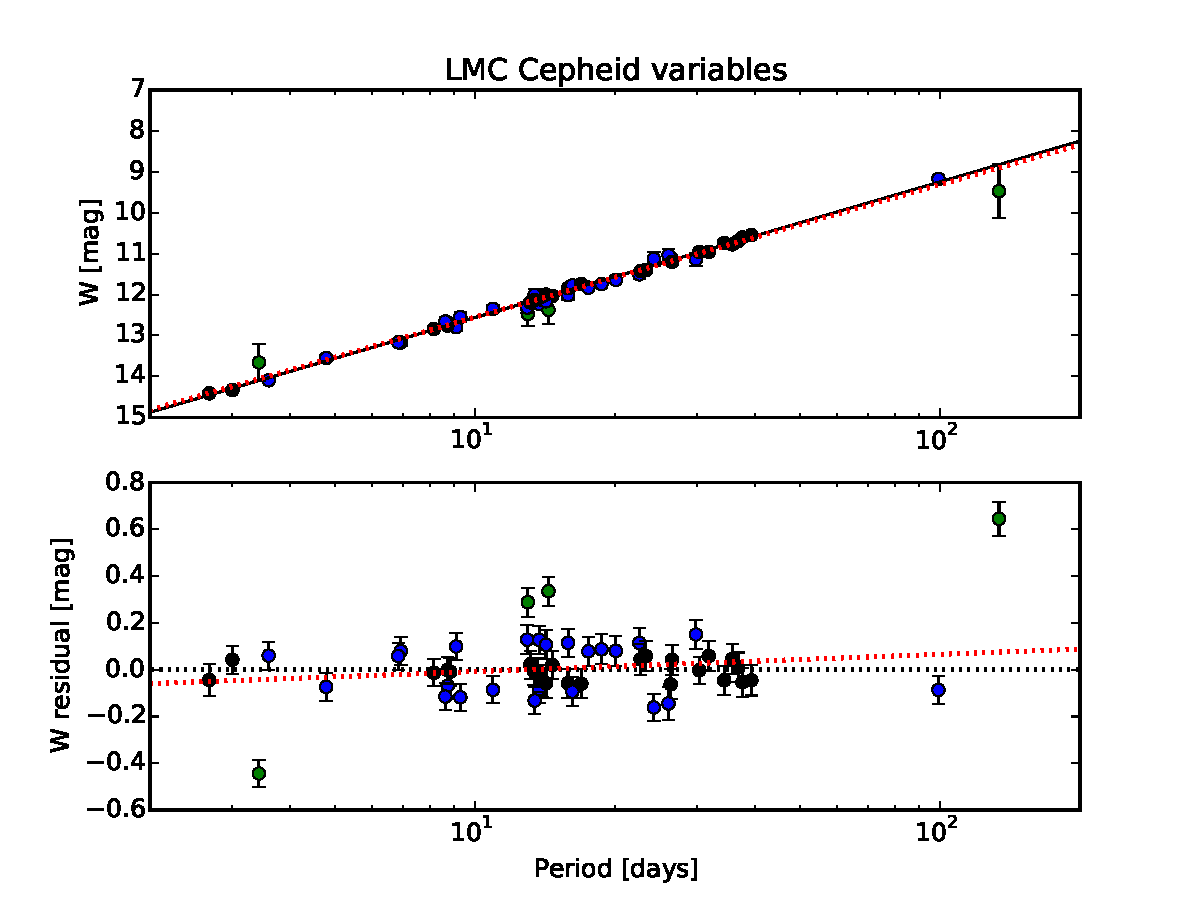
\includegraphics[scale=0.5]{../Draft/effective_HP_cepheids_LMC.pdf} }
\only<2>{
\begin{table}[tbp]
\centering
\begin{tabular}{@{}ccccc}
\hline
\multicolumn{5}{c}{LMC Cepheid variables} \\
\hline
Fit & $A$ & $b_W$ & $\sigma_{\intt}^{\LMC}$ & Period cut \\
\hline
 a & $12.570\,(0.035)$ & $-3.32\,(0.10)$ & $0.06$ & $10<P<60$ \\
  
 b & $12.562\,(0.016)$&$-3.30\,(0.05)$ & $0.06$ & $P<60$ \\

 c & $12.562\,(0.016)$& $-3.31\,(0.05)$& $0.06$ & $P<205$ \\

 d & $12.555\,(0.019)$& $-3.24\,(0.06)$& $0.12$ & $P<205$ \\
\hline
\end{tabular}
\end{table}

\begin{equation*}
\mu_{0,\LMC}^{\rm M} = 18.49 \pm 0.05, \quad M_W = -5.93 \pm 0.07
\end{equation*}
}
\end{frame}

\begin{frame}{Applying HP}{Milky Way (MW)}
\centering
MW figure
%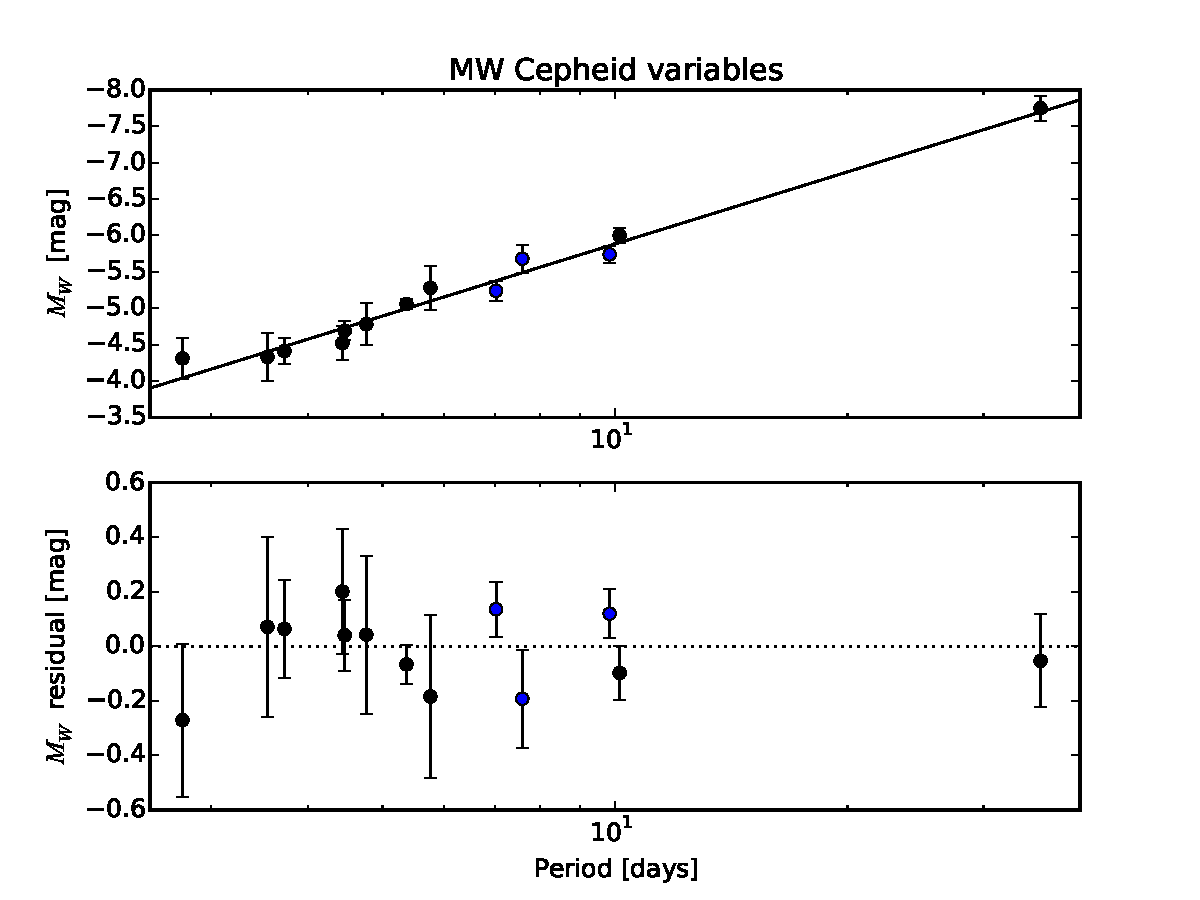
\includegraphics[scale=0.45]{../Draft/effective_HP_cepheids_MW.pdf}
\begin{equation*}\label{Eq:MW-bestfit}
M_W = -5.88 \pm 0.07  , \qquad b_W = -3.30 \pm 0.26  , \qquad \sigma_{\intt}^{\MW} = 0.02 ,
\end{equation*}
\end{frame}

\begin{frame}{Applying HP}{Megamaser system NGC 4258}
\only<1>{4258 figure%\centering
%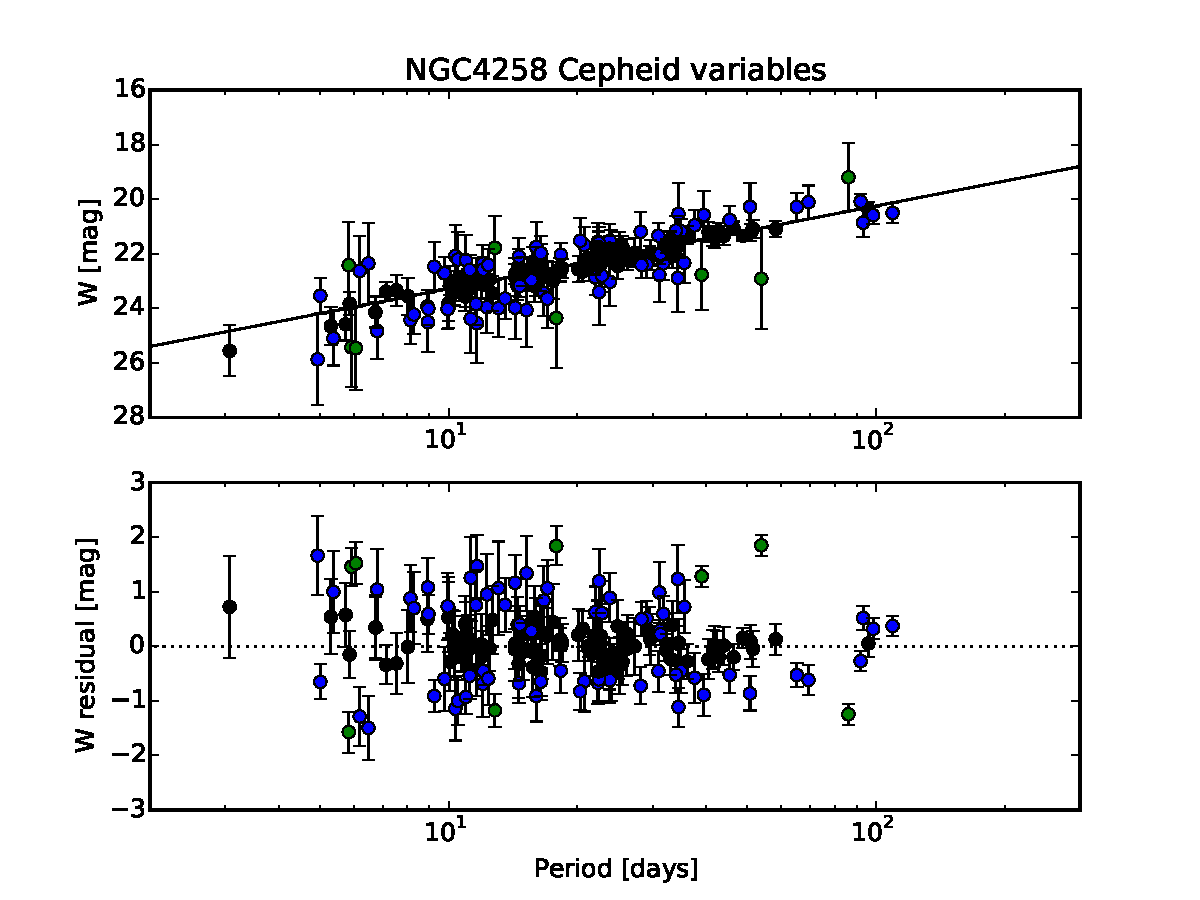
\includegraphics[scale=0.45]{../Draft/effective_HP_cepheids_NGC4258.pdf}
\begin{equation*}
\mu_{0,\rm 4258} = 29.40 \pm 0.07, \qquad M_W=-6.12 \pm 0.15, \quad b_W = -3.02 \pm 0.17  , \qquad \sigma_{\intt}^{\rm NGC4258} = 0.12 .
\end{equation*} }
\only<2>{\centering
I do not see any reason to discard those data sets }
\end{frame}

\section{The Hubble constant $H_0$}

\begin{frame}{The Hubble constant $H_0$}{Data}
\begin{itemize}
\item 8 SN Ia hosts: apparent magnitudes
\item MW Cepheid variables (parallax measurements): period, metallicity, magnitudes
\item LMC Cepheid variables: period, metallicity, magnitudes
\item Distance modulus to LMC derived from eclipsing binaries
\item Distance modulus to NGC 4258 derived from geometric maser distance and from standardised candle method for type IIP SNe   
\end{itemize}  
%\begin{columns}
%\begin{column}{0.45\textwidth}
%\centering
%\only<1-4>{Gaussian, isotropic simulation
%\includegraphics[scale=0.2]{../../../../../projects/B/ksv-maps/planck-nside/gaussian/192c/vmap_2000.pdf}} 
%\end{column}
%\begin{column}{0.45\textwidth}
%\centering 
%\only<2-3>{Inpainted SMICA 
%\includegraphics[scale=0.2]{../../../../../projects/B/ksv-maps/planck-nside/smica/192c/inpainted/vmap.pdf}}
%\only<4>{Inpainted NILC 
%\includegraphics[scale=0.2]{../../../../../projects/B/ksv-maps/planck-nside/nilc/192c/inpainted/vmap.pdf}}
%\end{column}
%\end{columns}
\end{frame}

\begin{frame}{The Hubble constant $H_0$}{The likelihood}
\begin{itemize}
\item Full likelihood 
\begin{equation*}
\ln P(\vec{w},\lbrace D_i \rbrace) = \ln P^{\Cepheid} + \ln P^{\SNe} + \ln P^{\Anchors}. 
\end{equation*}
\item For instance
\begin{equation*}
\ln P^{\Cepheid} = \sum_{ij} \ln \tilde{\chi}^{2}(\chi^{2,\Cepheid}_{ij}) + \ln \tilde{N}^{\Cepheid}_{ij},
\end{equation*}
\item $\SNe$, $\Anchors$,...
%\begin{equation*}
% \ln P^{\SNe} = \sum_{i} \ln \tilde{\chi}^{2}(\chi^{2,\SNe}_{i}) + \ln \tilde{N}^{\SNe}_{i} - \frac{(a^{R11}_v - a_v)^2}{2 \sigma_{a_v}^2} - \frac{\ln (2\pi\sigma_{a_v}^2)}{2} - \frac{(a_{\rm cal})^2}{2 \sigma_{a_{\rm cal}}^2} - \frac{\ln (2\pi\sigma_{a_{\rm cal}}^2)}{2}
%\end{equation*}
\end{itemize}
%\begin{columns}
%\begin{column}{0.45\textwidth}
%\centering
%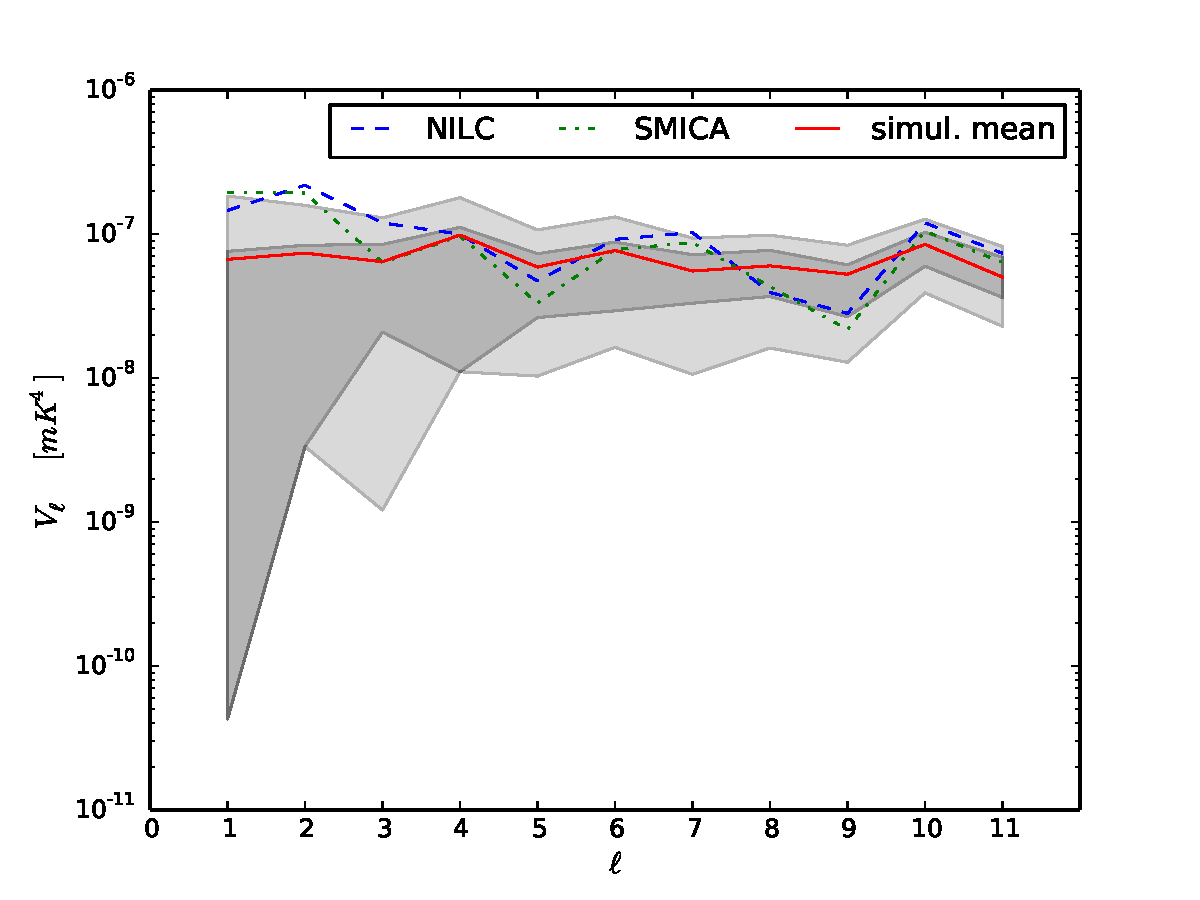
\includegraphics[scale=0.3]{../../../../../projects/B/ksv-spectra/planck-nside/plots/inpainted/192c/Inp_Vl.pdf} 
%\end{column}
%\begin{column}{0.45\textwidth}
%\centering 
%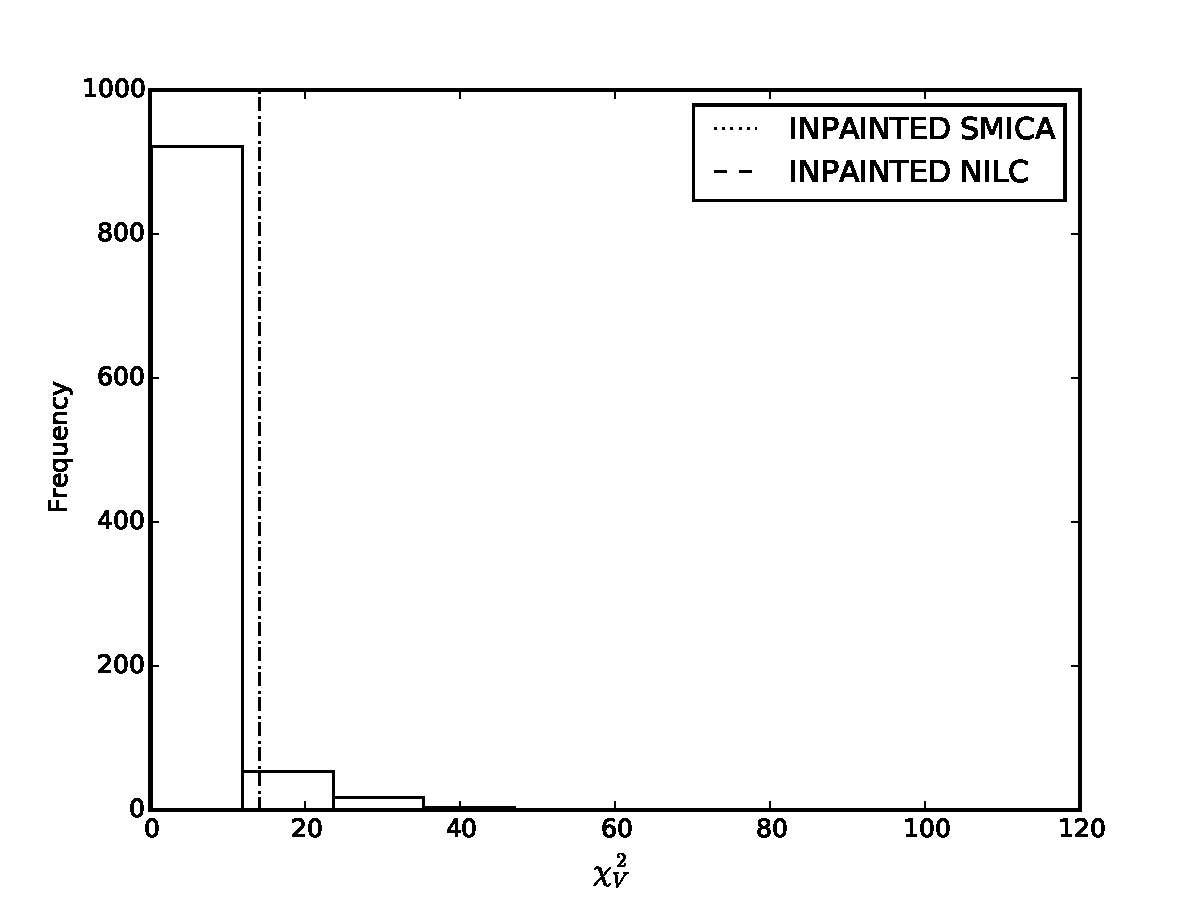
\includegraphics[scale=0.3]{../../../../../projects/B/ksv-spectra/planck-nside/plots/inpainted/192c/vchi2.pdf} 
%\end{column}
%\end{columns}
\end{frame}

\begin{frame}{The Hubble constant $H_0$}{Results}
\begin{table}[tbp]
\centering
\begin{tabular}{@{}lcccccr}
\hline
\multicolumn{7}{c}{NGC $4258 +$ LMC $+$ MW anchors} \\
\hline
Fit & $H_0$ & $M_W$ & $b_W$ & $Z_W$ &$\sigma_{\intt}^{\LMC}$ & $\sigma_{\intt}^{\MW}$\\
\hline
$M1^{a}$ & $75.0\,(3.9)$ & $-5.87\,(0.18)$ & $-3.20\,(0.05)\,[N]$ & $-0.005\,(0.020)\,[S]$ & $0.06$& $0.02$ \\
$M1^{af}$ & $74.9\,(3.9)$ & $-5.88\,(0.18)$ & $-3.20\,(0.05)\,[N]$ & $-0.005\,(0.020)\,[S]$ & $0.06$& $0.02$ \\
$M1^{ag}$ & $73.3\,(2.4)$ & $-5.88\,(0.18)$ & $-3.19\,(0.05)\,[N]$ & $-0.004\,(0.020)\,[S]$ & $0.06$& $0.02$ \\
$M1^{ah}$ & $74.6\,(1.9)$ & $-5.89\,(0.17)$ & $-3.21\,(0.05)\,[N]$ & $-0.005\,(0.020)\,[S]$ & $0.06$& $0.02$ \\
$M1^{aj}$ & $72.4\,(2.2)$ & $-5.90\,(0.18)$ & $-3.20\,(0.05)\,[N]$ & $-0.004\,(0.020)\,[S]$ & $0.06$& $0.02$ \\
$M1^{b}$ & $76.1\,(3.1)$ & $-5.86\,(0.17)$ & $-3.27\,(0.04)\,[N]$ & $-0.007\,(0.019)\,[S]$ & $0.06$ & $0.02$ \\
$M1^{be}$ & $75.1\,(3.4)$ & $-5.89\,(0.18)$ & $-3.25\,(0.07)\,[N]$ & $-0.004\,(0.020)\,[S]$ & $0.113$ & $0.10$ \\
$M2^{a}$ & $74.7\,(4.0)$ & $-4.68\,(0.97)$ & $-3.20\,(0.05)\,[N] $ & $-0.141\,(0.110)\,[W] $ & $0.06 $ & $0.02 $ \\
$M2^{b}$ & $ 75.1\,(3.8)$ & $-3.84\,(1.05)$ & $-3.28\,(0.04)\,[N]$ & $-0.236\,(0.119)\,[W]$ & $0.06$ & $0.02$ \\
$M3^{a}$ & $75.0\,(3.9)$ & $-5.92\,(0.04)$ & $-3.20\,(0.05)\,[N]$ & $0$ & $0.06$ & $0.02$ \\
$M3^{b}$ & $75.4\,(3.7)$ & $-5.92\,(0.04)$ & $-3.27\,(0.04)\,[N]$ & $ 0 $ & $0.06$ & $0.02$ \\
$M4^{a}$ & $74.7\,(4.0)$ & $-4.35\,(1.11)$ & $-3.20\,(0.05)\,[N]$ & $-0.178\,(0.125)\,[N]$ & $0.06$ & $0.02$ \\
$M4^{b}$ & $75.2\,(3.9)$ & $-3.18\,(1.25)$ & $-3.28\,(0.04)\,[N]$ & $-0.311\,(0.141)\,[N]$ & $0.06$ & $0.02$ \\
\hline

\end{tabular}

\end{table}
%\begin{columns}
%\begin{column}{0.45\textwidth}
%\centering
%\only<1-4>{Gaussian, isotropic simulation
%\includegraphics[scale=0.2]{../../../../../projects/B/ksv-maps/planck-nside/gaussian/192c/smap_2000.pdf}} 
%\end{column}
%\begin{column}{0.45\textwidth}
%\centering 
%\only<2-3>{Inpainted SMICA 
%\includegraphics[scale=0.2]{../../../../../projects/B/ksv-maps/planck-nside/smica/192c/inpainted/smap.pdf}}
%\only<4>{Inpainted NILC 
%\includegraphics[scale=0.2]{../../../../../projects/B/ksv-maps/planck-nside/nilc/192c/inpainted/smap.pdf}}
%\end{column}
%\end{columns}
\end{frame}

\begin{frame}{The Hubble constant $H_0$}{Results: fit $M1^a$}

%\begin{columns}
%\begin{column}{0.45\textwidth}
\begin{figure}
Triangle plot
%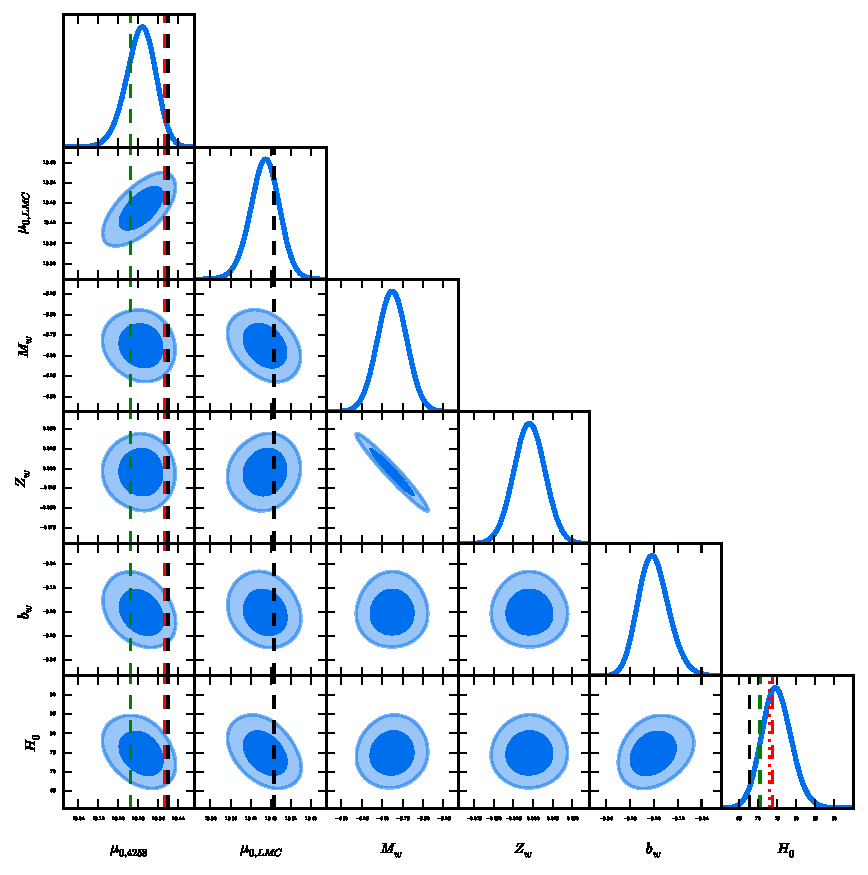
\includegraphics[scale=0.5]{../Draft/triangle_plot.pdf} 
\end{figure}

%\end{column}
%\begin{column}{0.45\textwidth}
%\centering 
%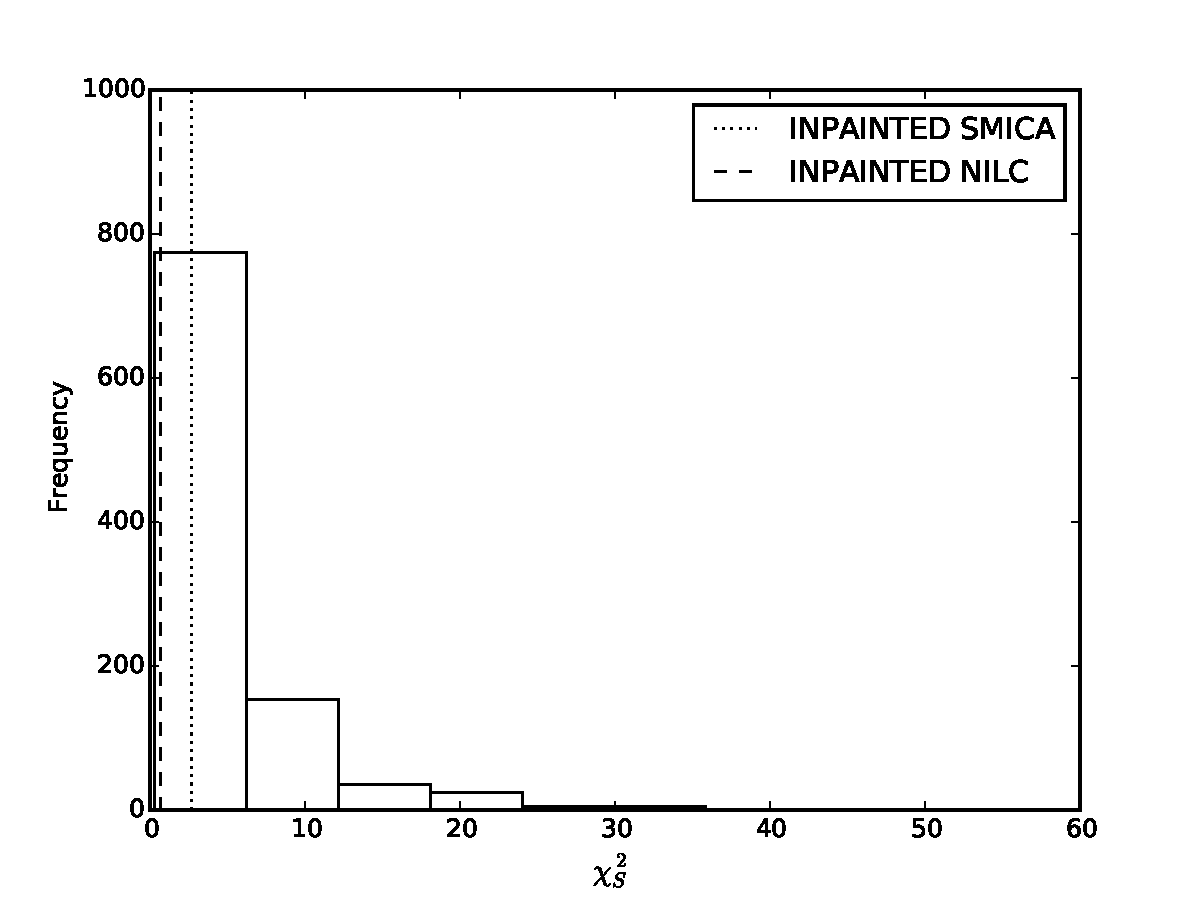
\includegraphics[scale=0.3]{../../../../../projects/B/ksv-spectra/planck-nside/plots/inpainted/192c/schi2.pdf} 
%\end{column}
%\end{columns}
\end{frame}

\begin{frame}{The Hubble constant $H_0$}{Conclusions}
\begin{itemize}
\item If one trust no one (HPs everywhere) $H_0=75.0\pm3.9$ a $5\%$ measurement.
\item Trust only distance modulus (no HPs) $H_0=74.6\pm1.9$  ($2.5\%$)
\item Trust only SN Ia $H_0=73.3\pm2.4$ ($3.3\%$)
\item Distrust both SN Ia and distance modulus data $H_0=72.4\pm2.2$  ($3\%$) 
\item Anchors choice: no reason to discard data
\item Metallicity: cannot say much about this with available data
\item Period cut: does not matter in our method
\item Results agree with R16: 18 SN Ia hosts, better distance modulus to NGC4258, consistent values of $H_0$, no outlier rejection needed any longer (they claim), no outliers among SN Ia hosts
%\item Do not reject data, keep the data and study the physics! (Adam Riess)
\end{itemize}
\end{frame}

\begin{frame}{The Hubble constant $H_0$}{Conclusions}
H0 valuess
%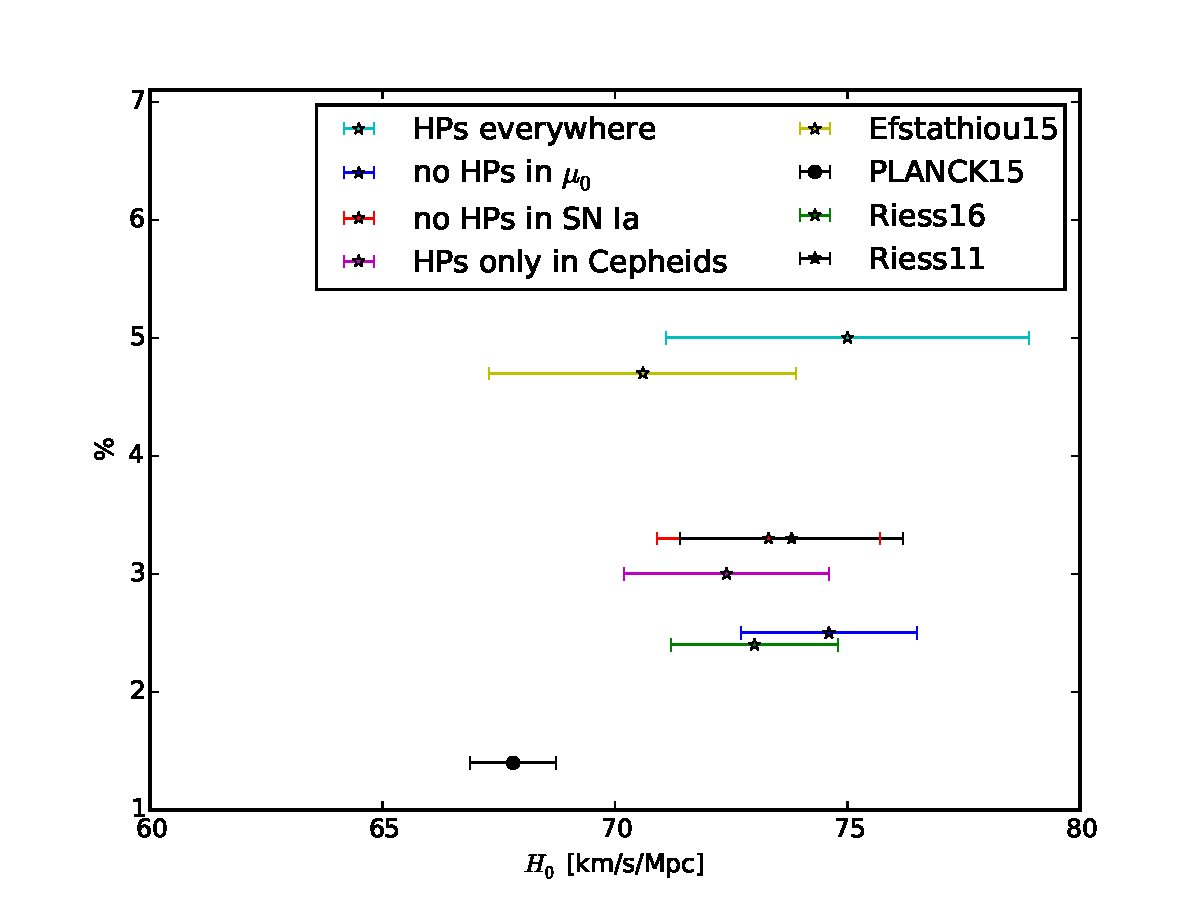
\includegraphics[scale=0.5]{./H0_values_2.pdf} 
\end{frame}
%\begin{columns}
%\begin{column}{0.45\textwidth}
%\centering
%\only<1-4>{Gaussian, isotropic simulation
%\includegraphics[scale=0.2]{../../../../../projects/B/ksv-maps/planck-nside/gaussian/192c/kmap_2000.pdf}} 
%\end{column}
%\begin{column}{0.45\textwidth}
%\centering 
%\only<2-3>{Inpainted SMICA 
%\includegraphics[scale=0.2]{../../../../../projects/B/ksv-maps/planck-nside/smica/192c/inpainted/kmap.pdf}}
%\only<4>{Inpainted NILC 
%\includegraphics[scale=0.2]{../../../../../projects/B/ksv-maps/planck-nside/nilc/192c/inpainted/kmap.pdf}}
%\end{column}
%\end{columns}
%\end{frame}


\end{document}



